\documentclass[twocolumn]{aastex631}
\usepackage{mathtools}
\usepackage{natbib}
\bibliographystyle{abbrvnat}
\setcitestyle{authoryear,open={(},close={)}}
\usepackage{txfonts}
\usepackage{lipsum, babel}
\usepackage[T1]{fontenc}
\usepackage{ae,aecompl}
\usepackage{xcolor,colortbl}
\usepackage{tikz}
\usepackage{graphicx}
\usepackage{url}
\usepackage{subfigure}
\usepackage{float}
\usepackage{amsmath}
\usepackage{amssymb}
\usepackage{cleveref}
\usepackage{physics}
\usepackage{empheq}
\usepackage{booktabs}
\usepackage{array}
\newcolumntype{R}[1]{>{\raggedleft\arraybackslash}p{#1}}
\newcolumntype{L}[1]{>{\raggedright\arraybackslash}p{#1}}
\usepackage{multirow}
\usepackage[flushleft]{threeparttable}
\usepackage{mathrsfs}
\usepackage{soul}
\pdfminorversion=5

\newcommand{\MyDiamond}[1][fill=black]{
\begin{tikzpicture}[x=1.2ex,y=1.2ex,line width=.1ex,line join=round, yshift=0.0ex] \draw  [#1]  (0,.5) -- (.5,1) -- (1,.5) -- (.5,0);
\end{tikzpicture}
}

\newcommand{\MyPlus}[1][fill=black]
{
\begin{tikzpicture}[x=1.5ex,y=1.5ex,line width=0.5ex]
\draw[#1] (0,.5) -- (1,.5);
\draw[#1] (.5,0) -- (.5,1);
\end{tikzpicture}
}

\newcommand{\MyCross}[1][fill=black]
{
\begin{tikzpicture}[x=1.ex,y=1.ex,line width=0.5ex]
\draw[#1] (0,0) -- (1,1);
\draw[#1] (0,1) -- (1,0);
\end{tikzpicture}
}

\newcommand{\MyTriangle}[1][fill=black]
{
\begin{tikzpicture}[x=1.ex,y=1.ex,line width=0.2ex]
\draw[#1] (0,1) -- (1,1);
\draw[#1] (1,1) -- (.5,0);
\draw[#1] (.5,0) -- (0,1);
\fill[#1] (0,1) -- (1,1) -- (.5,0) -- cycle;
\end{tikzpicture}
}

\newcommand{\MySolidLine}[1][fill=black]
{
\begin{tikzpicture}[x=2.ex,y=1.ex,line width=0.5ex]
\draw[#1] (0,.5) -- (2.5,.5);
\end{tikzpicture}
}

\newcommand{\MyDashedLine}[1][fill=black]
{
\begin{tikzpicture}[x=2.ex,y=1.ex,line width=0.5ex]
\draw [#1,dashed] (0,.5) -- (2.5,.5);
\end{tikzpicture}
}

\newcommand{\MyDashedDottedLine}[1][fill=black]
{
\begin{tikzpicture}[x=2.ex,y=1.ex,line width=0.5ex]
\draw [#1,dash dot] (0,.5) -- (2.5,.5);
\end{tikzpicture}
}

\newcommand{\MyDottedLine}[1][fill=black]
{
\begin{tikzpicture}[x=2.ex,y=1.ex,line width=0.5ex]
\draw [#1,dotted] (0,.5) -- (2.5,.5);
\end{tikzpicture}
}

\definecolor{Gray}{gray}{0.85}

\begin{document}
\title{The vertical Fermi and eROSITA bubbles inclined jets: A proof-of-concept study}


\author[0000-0002-1868-0660]{Po-Hsun Tseng}
\affiliation{Institute of Astrophysics, National Taiwan University, Taipei 10617, Taiwan}

\author[0000-0003-3269-4660]{H.-Y. Karen Yang}
\affiliation{Institute of Astronomy and Department of Physics, National Tsing Hua University, Hsinchu 30013, Taiwan}

\author[0000-0002-1249-279X]{Hsi-Yu Schive}
\affiliation{Institute of Astrophysics, National Taiwan University, Taipei 10617, Taiwan}
\affiliation{Department of Physics, National Taiwan University, Taipei 10617, Taiwan}
\affiliation{Center for Theoretical Physics, National Taiwan University, Taipei 10617, Taiwan}
\affiliation{Physics Division, National Center for Theoretical Sciences, Taipei 10617, Taiwan}

\author[0000-0003-2654-8763]{Tzihong Chiueh}
\affiliation{Institute of Astrophysics, National Taiwan University, Taipei 10617, Taiwan}
\affiliation{Department of Physics, National Taiwan University, Taipei 10617, Taiwan}
\affiliation{Center for Theoretical Physics, National Taiwan University, Taipei 10617, Taiwan}


\correspondingauthor{Po-Hsun Tseng}
\email{zengbs@gmail.com}


\keywords{keywords}

\begin{abstract}
\begin{enumerate}
  \item Release the caveat of jet direction.
  \item Rule out the hadronic process.
  \item Predict the small inner bubbles.
  \item How to explain why we assume e\_CR << e\_gas
  \item How to explain the lifespan of bubbles is too long.
  \item How to explain the jet power.
  \item How to explain the inconsistant of gamma-ray map.
\end{enumerate}
\end{abstract}

\section{Introduction}


\section{Methodology}

  We used the GPU-accelerated special relativistic hydrodynamics AMR code (\textsc{gamer-sr}) developed at the\
  National Taiwan University\
  (Schive et al. \citeyear{gamer-1}, \citeyear{gamer-2}; \citeauthor{tseng2021} \citeyear{tseng2021})\
  to carry out the simulations of the Fermi and eROSITA bubbles by CR and relativistic fluid injections from the GC.

  The CRs are advected with the thermal gas, and in return the velocities of gas\
  can react to the gradients of the CR pressure via the source term\
  containing spatial divergence of fluid velocities.\

  Although the high-energy CRe ($10$ --- $100$ GeV) plays a crucial role in reproducing the $\gamma$-ray map\
  within the range of $1$ --- $100$ GeV, we assume the pressure of CRe is much less than that of gas\
  throughout the simulation so that we , and the Fermi bubbles can be outlined against the eROSITA bubbles.

  As stressed by \citet{Yang2012}, CR diffusion has insignificant effect on the overall morphology of the Fermi bubbles,\
  but only sharpens the edges of the simulated bubbles by the interplay between anisotropic CR diffusion\
  and magnetic fields with suppressed perpendicular diffusion across the bubble surface. Moreover,\
  the bubbles should be weak due to adiabatic expansion, and thus the magnetic fields has\
  little effect on the overall dynamics. For these two reasons,\
  we have ignored the CR diffusion and the magnetic field throughout\
  the simulation.

  We do not simulate the spectral evolution of the CR, and we neglected the cooling and heating processes of CRs,\
  such as energy losses due to synchrotron and inverse Compton emission, and reacceleration in shocks.\

  In this approach, we treat CRs as a single species without distinction between electrons and protons,\
  that cannot react to the gas via the application of CRe pressure,\
  and solve directly for the evolution of CR energy density $e_{\text{cr}}$\
  as a function of $\mathbf{r}$ and $t$.\

  Since the relativistic fluid ejected by the jet source\
  is quickly stalled off and slowed down by a dense ISM disk in a short time,\
  and the relativistic fluid\
  accounts for a little minority of total mass inside the simulation box,\
  we still use the Newtonian gravity to attack this problem.

  The governing equations solving the special relativistic ideal fluid\
  including CR advection, and dynamical coupling between the thermal gas and CRs without CR diffusion\
  turn out to be


  \begin{subequations}
    \label{governing-eq}
    \begin{align}
     &\partial_{t} D+\partial_{j} \left(DU^{j}/\gamma\right)=0,\label{D evolution}\\
     &\partial_{t} M^{i}+\partial_{j} \left(M^{i}U^{j}/\gamma+p_{\text{gas}}\delta^{ij}\right)=\
     -\rho\partial_{i}\Phi,\label{M evolution}\\
     &\partial_{t} \tilde{E}+\partial_j \left[\left(\tilde{E}+p_{\text{gas}}\right)U^{j}/\gamma\right]=0, \label{E evoltion}\\
     &\partial_{t} \left(\gamma e_{\text{cr}}\right) + \partial_{j} \left(e_{\text{cr}}U^{j}\right)=\
     -p_{\text{cr}} \partial_{j} U^{j},\label{D evolution}
    \end{align}
  \end{subequations}


  where the five conserved quantities of gas $D$, $M^{i}$, and $\tilde{E}$ are the mass density,\
  the momentum densities, and the reduced energy density, respectively.\
  The reduced energy density is defined by subtracting the rest mass energy density of gas\
  from the total energy density of gas.\
  $\gamma$ and $U^{j}$ are the temporal and spatial component of four-velocity of gas.\
  $\rho$ is the gas density in the local rest frame defined by $D/\gamma$.\
  $p_{\text{gas}}$ is the gas pressure.\
  $p_{\text{cr}}$ and $e_{\text{cr}}$ are the CR pressure and CR energy density measured in the local rest frame.\
  $\Phi$ is the gravitation potential.\
  $c$ is the speed of light, and $\delta^{ij}$ is the Kronecker delta notation.\
  Throughout this paper, Latin indices run from 1 to 3, except when stated otherwise.\

  The set of \Cref{governing-eq} is closed by using the Taub-Mathews equation of state (\citealt{Taub}; \citealt{TM_EOS})\
  that approximates the exact EoS \citep{Synge} for ultra-relativistically\
  hot gases coexisting with non-relativistically cold gases.

  \textsc{gamer-sr} adopts a new algorithm \citep{tseng2021} to convert between\
  primitive ($\rho$, $U^{j}$, $p$) and conserved variables ($D$, $M^{j}$, $\tilde{E}$),\
  significantly reducing numerical error caused by catastrophic cancellations\
  that commonly occur within the regions with high Mach number flows. e.g., jet-ISM interaction zones.

  \textsc{gamer-sr} also adaptively and locally reduce the min-mod coefficient\
  \citep{tseng2021} within the failed patch group.\
  Doing so provides an elegant way to avoid the use of pressure/density floor,\
  being unnatural but widely used in almost publicly available codes.\

  \subsection{The Galactic and Disk Models}
  As a proof-of-concept study, we approximate conventionally axisymmetric stellar potential of Milky Way\
  by an external plane-parallel potential that is symmetric about the mid-plane $z=0$\
  in a simulation box size of\
  $14\times14\times28$ kpc, slightly larger than the size of eROISTA bubbles.

  The plane-parallel potential is fixed throughout our simulations and given by
  \begin{equation}
    \Phi_{\text{total}}(z) = \Phi_{\text{bulge}}(z) + \Phi_{\text{halo}}(z),
  \end{equation}
  where
  \begin{equation}
    \Phi_{\text{bulge}}(z)=\
    2\sigma^2_{\text{bulge}}\
    \ln\cosh\left(z\sqrt{\frac{2\pi G\rho_{\text{bulge}}^{\text{peak}}}{\sigma^2_{\text{bulge}}}}\right)
  \end{equation}
  is the potential of an isothermal slab mainly contributed by stars around the Galactic bulge, and\
  $\Phi_{\text{halo}}(z)=v^2_{\text{halo}}\ln\left(z^2+d^2_{\text{h}}\right)$\
  is a plane-parallel dark logarithmic halo potential.

  With the help of the isothermal and hydrostatic equilibrium conditions,\
  and assuming the interface between isothermal disk and atmosphere is in pressure equilibrium,\
  we can write the steady-state gaseous density distributions,\
  confined in the total potential, of the disk and the Galactic atmosphere as\
  \begin{subequations}
  \begin{align}
     \displaystyle \rho_{\text{isoDisk}}(z) = \rho_{\text{isoDisk}}^{\text{peak}}
     \exp\left[-\frac{\Phi_{\text{total}}(z)}{k_{B}T_{\text{isoDisk}}/m_{\text{p}}}\right]&\label{isothermal-disk-density}\\
     \text{, if $|z| < z_{0}$}& \nonumber \\
     \nonumber\\
     \displaystyle \rho_{\text{atmp}}(z) = \rho_{\text{atmp}}^{\text{peak}}
     \exp\left[-\frac{\Phi_{\text{total}}(z)}{k_{B}T_{\text{atmp}}/m_{\text{p}}}\right]&\label{isothermal-atmp-density}\\
     \text{, otherwise,}& \nonumber
  \end{align}
  \label{disk-atm-sys}
  \end{subequations}
  where $m_{\text{p}}$ is the proton mass,\
  $T_{\text{isoDisk}}$ and $T_{\text{atmp}}$ is the temperature of the isothermal disk and atmosphere,\
  $\rho_{\text{isoDisk}}^{\text{peak}}$ and $\rho_{\text{atmp}}^{\text{peak}}$ is the peak mass density\
  of the disk and atmosphere on the mid-plane $z=0$.

  We tabulate parameters in the first four\
  categories of \Cref{table-parameters},\
  except for $\rho_{\text{atmp}}^{\text{peak}}$ that\
  can be derived from the known parameters and pressure equilibrium condition\
  on the interfaces $(z=\pm z_{0})$ between the disk and atmosphere.\

  The initial density profile of \Cref{disk-atm-sys} is shown in \Cref{density-profile}\
  and compared to the observed result \citep{Miller_2013} beyond 1 kpc.\

  Note that there is an difficulty in disentangling the contribution\
  of the Local Bubble, a supernova remnant in which the Solar System is embedded \citep{Snowden1990},\
  and the contribution from solar wind charge-exchange processes, which produce soft\
  X-ray emission throughout the Solar System. As a result, the density profile of the Galactic halo remains unclear\
  \citep{BlandHawthorn2016}.


  \begin{figure*}[h]
    \subfigure[The initial gaseous density profile along z-axis] % caption
    {
      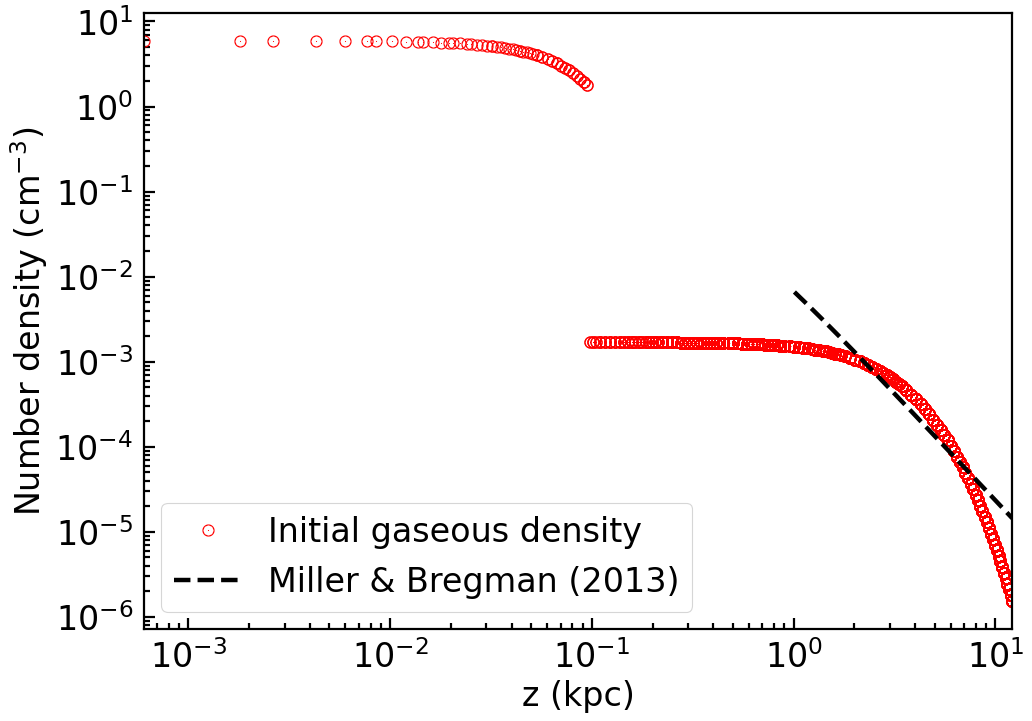
\includegraphics[width=0.4\linewidth]{figures/fig__density-profile.png}
      \label{density-profile}
    }
  \caption{Captions}
  \end{figure*}


  The AMR base level is covered by $16\times16\times32$ root grids, refined progressively on the plane $z=0$\
  , with the outflow boundary condition.


  \subsubsection{The clumpy, and warm/cold ISM disk}

  A crucial component in our work is the clumpy ISM disk initialized by\
  the publicly available pyFC code
  \footnote{\url{https://pypi.python.org/pypi/pyFC}}.
  First, pyFC creates a dimensionless 3D scalar field $f_{\text{clumpy}}(\bold{x})$ that is clumpy but obeys\
  the log-normal probability distribution\
  %the log-normal probability distribution \citep{Berkhuijsen2008}\
  with mean $\mu_{\text{clumpy}}$ and dispersion $\sigma_{\text{clumpy}}$,\
  and follows the power-law Kolmogorov spectrum
  \begin{equation}
    D(\bold{k})=\int k^{2} \hat{f}(\bold{k})\hat{f}^{*}(\bold{k})d\Omega \propto k^{-\beta},
    \label{Kolmogorov-spectrum}
  \end{equation}
  where $\hat{f}(\bold{k})$ is the Fourier transform of $f_{\text{clumpy}}(\bold{x})$.\
  The spectrum $D(\bold{k})$ in the Fourier space is characterized by the power law index $\beta$,\
  the Nyquist limit $k_{\text{max}}$, and the lower cutoff wave number $k_{\text{min}}$.
  $k_{\text{max}}$ is one-half of the spatial resolution within disk,\
  and $k_{\text{min}}$ is 375.0, corresponding to the maximum size of an individual clump $\sim 20$ pc.\


  The temperature in each cell of the clumpy disk is determined by $p_{\text{disk}}$


  We summarize the parameters of clumpy disk and their references in \Cref{table-parameters}.



  %The reader is referred to \citet{LA2002} and \citet{Wagner2012} for further details of this method.
  \citet{LA2002} and \citet{Wagner2012} have outlined a detailed procedure\
  for constructing clumpy structure, and we do not repeat here.


  The temperature in each cell of the warm gas distribution is determined by pressure equilibrium with hot gas.\
  When the warm gas temperature exceeds $T_{\text{crit}}=$ K, it is deemed to be thermally unstable and is replaced\
  by hot gas. This makes the gas porous.


  \begin{enumerate}
     \item Constructing the isothermal disk $\rho_{\text{isoDisk}}(\bold{x})$ by \Cref{isothermal-disk-density}.
     \item Using PyFC code to obtain a dimensionless clumpy distribution $f_{\text{clumpy}}$ obeying\
           lognormal distribution and the power-law spectrum, \Cref{Kolmogorov-spectrum}.
     \item $\rho_{\text{ismDisk}}(\bf{x}) = f_{\text{clumpy}}(\bf{x}) \rho_{\text{isoDisk}}(\bf{x})$.
     \item
  \end{enumerate}


% Please add the following required packages to your document preamble:
% \usepackage{booktabs}
\begin{table*}[t]
\centering
\caption{Parameters of the disk, atmosphere, and gravitational potential in the simulation.}
\label{table-parameters}
\begin{tabular}{@{}llrc@{}}
\toprule[1pt]\midrule[0.3pt]
Parameter                                                    & Description                               & Value                                \\ \midrule
{\bf Static stellar potential }\citep{velocity-dispersion-MW}&                                           &                                      \\
$\sigma_{\text{bulge}}$                                      & Velocity dispersion of bulge              & 100 km$\cdot$s$^{-1}$                \\
$\rho_{\text{bulge}}^{\text{peak}}$                          & Peak average density of bulge             & $4\times 10^{-24}$ g$\cdot$cm$^{-3}$ \\ \hline
{\bf Static dark halo potential }\citep{Johnston1995}        &                                           &                                      \\
$v_{\text{halo}}$                                            &                                           & 131.5 km$\cdot$s$^{-1}$              \\
$d_{\text{h}}$                                               & Core radius                               & 12 kpc                               \\ \hline
{\bf Isothermal disk }\citep{peak-ism-density}               &                                           &                                      \\
$z_{0}$                                                      & Scale height of disk                      & 100 pc                               \\
$T_{\text{\text{isoDisk}}}$                                  & Temperature of disk                       & $10^{3}$ K                           \\
$\rho_{\text{isoDisk}}^{\text{peak}}$                        & Peak mass density of disk                 & $10^{-23}$ g$\cdot$cm$^{-3}$         \\ \hline
{\bf Atmosphere }\citep{temperature-MW}                      &                                           &                                      \\
$T_{\text{\text{atmp}}}$                                     & Temperature of atmosphere                 & $10^{6}$ K                           \\ \hline
{\bf Clumpy disk }\citep{Wagner2012}                         &                                           &                                      \\
$T_{\text{\text{c}}}$                                        & Critical temperature of warm atomic phase & $3\times 10^{4}$ K                   \\
$k_{\text{min}}$                                             & Cutoff wave number                        & 375.0                                \\
$\mu_{\text{clumpy}}$                                        & Mean of number density                    & 1.0 $\text{cm}^{-3}$                 \\
$\sigma_{\text{clumpy}}$                                     & Dispersion of number density              & 1.7 $\text{cm}^{-3}$                 \\ % RELATIVISTIC JET FEEDBACK IN EVOLVING GALAXIES Wagner (2011)
$\beta$                                                      & Power law index                           & -5/3                                 \\ \midrule
\end{tabular}
\end{table*}


\begin{enumerate}
  \item Assumptions on gravity:
    \begin{enumerate}
      \item We use the potential of isothermal slab, symmetric about $z=0$ and\
            supported by gas pressure and by under its own self-gravity,\
            to mimic the realistic potential of Galactic bulge.
      \item The ISM disk and atmosphere are subjected to the fixed external potential\
            due to a disk bulge and dark matter halo.
      \item In addition to the gravitational interaction, we ignore other interactions between stars and gases.
      \item We also ignore the self-gravity of the ISM disk and of the atmosphere.
      \item We ignore the centrifugal force of Milky Way rotation acting on the bubbles.
      \item We use the potential of isothermal slab to mimic the gravitational potential due to the stellar bulge.
      \item The interface between cold ISM disk and atmosphere is parallel to the Galactic plane and is pressure balanced.
    \end{enumerate}
\end{enumerate}



\begin{enumerate}
\item Fixed external gravitational potential:
  \begin{enumerate}
    \item Bulge potential:
      \begin{enumerate}
       \item Peak density: $\rho_{\text{bulge}}^{\text{peak}}=4\times 10^{-24}$ g/cm$^3$.
       \item Potential (isothermal slab):
         \begin{equation}
           \Phi_{\text{bulge}}=\
           2\sigma^2_{\text{bulge}}\
           \ln\cosh\left(z\sqrt{\frac{2\pi G\rho_{\text{bulge}}^{\text{peak}}}{\sigma^2_{\text{bulge}}}}\right),
         \end{equation}
          where $\displaystyle \sigma_{\text{bulge}}=\
                \sqrt{\frac{k_{B}T_{\text{bulge}}}{m}}=100$ km/s \citep{velocity-dispersion-MW}.
      \end{enumerate}

    \item Dark logarithmic halo potential:
         \begin{equation}
           \Phi_{\text{halo}}=v^2_{\text{halo}}\ln\left(z^2+d^2_{\text{h}}\right),
         \end{equation}
         where $v_{\text{halo}}=131.5$ km/s, $d_{\text{h}}=12$ kpc \citep{Yang2013}.

    \item Total potential: $\Phi_{\text{total}}=\Phi_{\text{bulge}}+\Phi_{\text{halo}}$.
  \end{enumerate}


\item Clumpy cold disk:
  \begin{enumerate}
    \item Dimension: $14\times14\times0.2$ kpc. i.e. Scale height, $z_{0}=100$ pc. \citep{peak-ism-density}
    \item Peak mass density: $\rho_{\text{disk}}^{\text{peak}}=10^{-23}$ g/cm$^3$. \citep{peak-ism-density}
    \item Average temperature: $T_{\text{disk}}=10^{3}$ K. \citep{peak-ism-density}
    \item Average mass density:
          \begin{equation}
             \rho_{\text{disk}}=\rho_{\text{disk}}^{\text{peak}}
             \exp\left[-\frac{\Phi_{\text{total}}}{k_{B}T_{\text{disk}}/m}\right].
             \label{disk-density}
          \end{equation}

    \item Pressure: $\displaystyle p_{\text{disk}}=\rho_{\text{disk}}T_{\text{disk}}$.

    \item The clumpy cuboid, using the publicly\
          available pyFC code\footnote{\url{https://pypi.python.org/pypi/pyFC}},\
          are described by a log-normal distribution with mean 1.0 and variance 5.0.\
          Also, the power spectrum of the clumpy cuboid is characterized by $k_{\text{min}}$ and $\beta$,\
          where $k_{\text{min}}$ sets the maximum cloud size within the clumpy cuboid,\
          and $\beta$ is the slope of power spectrum in Fourier space.
          In this paper, we set $\beta=-5/3$ and $k_{\text{min}}=375$ to follow the Kolmogorov spectrum\
          and to limits the maximum size of an individual cloud to approximately 25 pc.

    \item The clumpy disk is then constructed by multiplying a fractal cuboid with \Cref{disk-density}.

    \item The clouds and voids within clumpy disk are pressure balanced.
  \end{enumerate}


\item Isothermal atmosphere:
  \begin{enumerate}
     \item The region outside the clumpy cold disk is atmosphere.
     \item $T_{\text{atmp}}=10^{6}$ K. \citep{temperature-MW}
     \item Density:
          \begin{equation}
             \rho_{\text{atmp}}=\rho_{\text{atmp}}^{\text{peak}}
             \exp\left[-\frac{\Phi_{\text{total}}}{k_{B}T_{\text{atmp}}/m}\right],
             \label{atmosphere-density}
          \end{equation}
          where $\rho_{\text{atmp}}^{\text{peak}}$ can be obtained by assuming that pressure\
          and gravitational potential are continuous at the interface ($z=\pm z_{0}$) between disk and atmosphere.
  \end{enumerate}



\end{enumerate}

\subsection{Cold disk}
  We restrict the refinement level is 7 within the cold disk so that\
  a molecular cloud can be adequately resolved by approximately 30 cells along their diameter, 100 pc.\

\subsection{Jet injection}
  We resolve the jet source located at the center of the simulation domain,\
  cells are refined to level 11, leading to a finest spatial resolution of 0.4 pc.\

 \begin{enumerate}
    \item Why the overall structure is insensitive to jet direction?
      \begin{enumerate}
        \item Jet source size.
        \item Cold disk.
        \item Large pressure gradient along z-dircetion.
      \end{enumerate}
 \end{enumerate}



\subsection{X-ray and Gamma-ray emission}


  \begin{enumerate}
    \item X-ray:
       \begin{enumerate}
         \item Thermal bremsstrahlung: The X-ray emissivity in an energy range 1.4–1.6 keV is calculated\
               using the MEKAL model (\citealt{Xray-1}; \citealt{Xray-2}; \citealt{Xray-3})\
               implemented in the utility XSPEC\citep{XSPEC}, assuming solar metallicity.
       \end{enumerate}
    \item Gamma-ray:
       \begin{enumerate}
         \item Leptonic process:\\
          The gamma-ray emission is produced by inverse Comptom scattering of the ISRF by CRe.
         \item Hadronic process:\\
          In the hadronic model, CRp undergo hadronic collisions with thermal gas protons\
          and produce $\gamma$-ray via pion decay. The volume emissivity of the emission can be written as
          \begin{equation}
             \epsilon \propto U_{\text{CRp}}n_{p}\sigma_{p}\kappa_{pp}.
          \end{equation}
       \end{enumerate}
  \end{enumerate}



Note that the observed X-ray emission is contributed by all the gas in the Milky Way halo,\
which likely extends to a radius of $\sim$250 kpc (\citealt{halo-radius-1}; \citealt{halo-radius-2}),\
much bigger than our simulation box. Therefore, we first compute the X-ray emissivity\
from the simulated gas within a radius of 25 kpc away from the GC.
Then, beyond 25 kpc the gas is assumed to be isothermal with $T=10^6$ K and\
follows out to a radius of 250 kpc the observed density profile of \citep{temperature-MW}.

Inverse Compton scattering
\begin{equation}
  \frac{dE}{dtd\epsilon_{1}dV} = \frac{3}{4}\sigma_{T}c\textit{C}\epsilon_{1}\int^{\epsilon_{\text{max}}}_{\epsilon_{\text{min}}}
               \frac{n(\epsilon)}{\epsilon}d\epsilon\int^{\gamma_{\text{max}}}_{\gamma_{\text{min}}\left(\epsilon\right)}
               \gamma^{-(p+2)}f(q, \Gamma)d\gamma.
\end{equation}


\begin{equation}
f(\gamma_{\text{e}}, \epsilon) = 2q\ln q+(1+2q)(1-q)+0.5(1-q)\frac{\left(\Gamma q\right)^2}{1+\Gamma q},
\end{equation}

\begin{equation}
\Gamma=\frac{4\epsilon \gamma_{\text{e}}}{m_{\text{e}}c^2}
\end{equation}

$\gamma_{\text{min}}\left(\epsilon\right)$ is the root of $f(\gamma_{\text{e}}, \epsilon)=0$ at a specific incident photon energy.

\begin{equation}
q=\frac{\epsilon_{1}/\gamma_{\text{e}}m_{\text{e}}c^{2}}{\Gamma\left(1-\epsilon_{1}/\gamma_{\text{e}}m_{\text{e}}c^{2}\right)}.
\end{equation}


Hadronic process
\begin{equation}
  \frac{dE}{dtd\epsilon_{1}dV} = cn_{H}pC\left(\frac{\epsilon_{1}}{m_{\text{p}}c^2}\right)^{-p}\int_{0}^{1}\sigma(\epsilon_{\text{p}}) F(x,\epsilon_{\text{p}}) x^{p}dx.
\end{equation}

\begin{equation}
\sigma(\epsilon_{\text{p}})=34.3+1.88L+0.25L^{2}\left[1-\frac{E_{\text{threshold}}}{E_{\text{p}}}\right]^{4} \text{ mb}.
\end{equation}

\begin{equation}
F(x,\epsilon_{\text{p}})=B\frac{d}{dx}\left[\ln(x)\left(\frac{1-x^{\beta}}{1+kx^{\beta}\left(1-x^{\beta}\right)}\right)^4\right],
\end{equation}


where
$x=\epsilon_{1}/\epsilon_{\text{p}}$, $B=1.30+0.14L+0.011L^2$, $\beta=\left(1.79+0.11L+0.008L^{2}\right)^{-1}$,\
$\left(0.801+0.049L+0.014L^{2}\right)^{-1}$, $L=\ln(\epsilon_{\text{p}}/1 \text{ TeV})$.


\section{to-do-list}
\begin{enumerate}
  \item Predict cold inner bubbles, emitting OIII or OII spectrum.
\end{enumerate}

\section{conclusions}

\section*{Data Availability}
The data underlying this article are available in the article and in its online supplementary material.


%%%%%%%%%%%%%%%%%%%% REFERENCES %%%%%%%%%%%%%%%%%%
\bibliographystyle{mnras}
\bibliography{paper} % if your bibtex file is called example.bib

%%%%%%%%%%%%%%%%% APPENDICES %%%%%%%%%%%%%%%%%%%%%

\appendix

\end{document}
